\documentclass[a4paper,11pt,twoside]{book}

\usepackage{lmodern}
\usepackage[francais]{babel}
\usepackage{graphicx}

\usepackage{amssymb,amsmath}
\usepackage{ifxetex,ifluatex}
\usepackage{fixltx2e} % provides \textsubscript
\ifnum 0\ifxetex 1\fi\ifluatex 1\fi=0 % if pdftex
  \usepackage[T1]{fontenc}
  \usepackage[utf8]{inputenc}
\else % if luatex or xelatex
  \ifxetex
    \usepackage{mathspec}
  \else
    \usepackage{fontspec}
  \fi
  \defaultfontfeatures{Ligatures=TeX,Scale=MatchLowercase}
\fi
% use upquote if available, for straight quotes in verbatim environments
\IfFileExists{upquote.sty}{\usepackage{upquote}}{}
% use microtype if available
\IfFileExists{microtype.sty}{%
\usepackage{microtype}
\UseMicrotypeSet[protrusion]{basicmath} % disable protrusion for tt fonts
}{}


% load listing package
% and redefine the vebatim environment
\usepackage{listings}
\usepackage[T1]{fontenc}
\usepackage{color}
\definecolor{gray}{rgb}{0.7,0.7,0.7}
\lstset{
    basicstyle=\linespread{0.85}\footnotesize\ttfamily,
    literate=
    {á}{{\'a}}1 {é}{{\'e}}1 {í}{{\'i}}1 {ó}{{\'o}}1 {ú}{{\'u}}1
    {Á}{{\'A}}1 {É}{{\'E}}1 {Í}{{\'I}}1 {Ó}{{\'O}}1 {Ú}{{\'U}}1
    {à}{{\`a}}1 {è}{{\`e}}1 {ì}{{\`i}}1 {ò}{{\`o}}1 {ù}{{\`u}}1
    {À}{{\`A}}1 {È}{{\'E}}1 {Ì}{{\`I}}1 {Ò}{{\`O}}1 {Ù}{{\`U}}1
    {ä}{{\"a}}1 {ë}{{\"e}}1 {ï}{{\"i}}1 {ö}{{\"o}}1 {ü}{{\"u}}1
    {Ä}{{\"A}}1 {Ë}{{\"E}}1 {Ï}{{\"I}}1 {Ö}{{\"O}}1 {Ü}{{\"U}}1
    {â}{{\^a}}1 {ê}{{\^e}}1 {î}{{\^i}}1 {ô}{{\^o}}1 {û}{{\^u}}1
    {Â}{{\^A}}1 {Ê}{{\^E}}1 {Î}{{\^I}}1 {Ô}{{\^O}}1 {Û}{{\^U}}1
    {œ}{{\oe}}1 {Œ}{{\OE}}1 {æ}{{\ae}}1 {Æ}{{\AE}}1 {ß}{{\ss}}1
    {ű}{{\H{u}}}1 {Ű}{{\H{U}}}1 {ő}{{\H{o}}}1 {Ő}{{\H{O}}}1
    {ç}{{\c c}}1 {Ç}{{\c C}}1 {ø}{{\o}}1 {å}{{\r a}}1 {Å}{{\r A}}1
    {€}{{\euro}}1 {£}{{\pounds}}1 {«}{{\guillemotleft}}1
    {»}{{\guillemotright}}1 {ñ}{{\~n}}1 {Ñ}{{\~N}}1 {¿}{{?`}}1,
    tabsize=4,
    columns=fixed,
    numbers=left,
    stepnumber=1,
    numberstyle=\linespread{0.85}\tiny\color{gray},
    frame=leftline,
    framerule=0.1pt,
    rulecolor=\color{gray},
    frameround=tttt,
    framesep=3pt,
    numbersep=5pt,
    xleftmargin=1pt
}
\let\verbatim\relax
\lstnewenvironment{verbatim}[1][]{#1}{}


\usepackage{geometry}
\geometry{
  margin=1.5cm,
  footskip=1.5cm,
}


% define PDF format options
\usepackage{hyperref}
\hypersetup{ % configuration de hyperref
  draft=false,          		% true pour imprimer sans les liens
  bookmarks=true,       		% Signets
  bookmarksnumbered=true,   % Signets numérotés
  pdfpagemode=None,         % Signets/vignettes fermé à l'ouverture
  pdfstartview=FitH,        % La page prend toute la largeur
  pdfpagelayout=SinglePage, % Vue par page
  colorlinks=true,     			% Liens en couleur
  urlcolor=blue,     				% Couleur des liens externes
  pdfborder={0 0 0},        % Style de bordure : ici, pas de bordure
  pdfauthor={Patrick Fuchs et Pierre Poulain},
  pdftitle={Cours de Python},
  pdfsubject={Cours de Python},
  pdfkeywords={programmation,Python,biologie},
  pdfcreator={pandoc},
  pdfproducer={pandoc}
}


% define page header and footer
\usepackage{fancyhdr}
\pagestyle{fancy}
\fancyhf{} % clear all headers and footer fields
\fancyhead[LE,RO]{\nouppercase{\leftmark}}
\fancyhead[RE,LO]{\nouppercase{\rightmark}}
\fancyfoot[LE,RO]{\thepage}
\fancyfoot[RE,LO]{\it Cours de Python / Université Paris Diderot - Paris 7 / UFR Sciences du Vivant}



\hypersetup{unicode=true,
            pdfborder={0 0 0},
            breaklinks=true}
\urlstyle{same}  % don't use monospace font for urls


\usepackage{graphicx,grffile}
\makeatletter
\def\maxwidth{\ifdim\Gin@nat@width>\linewidth\linewidth\else\Gin@nat@width\fi}
\def\maxheight{\ifdim\Gin@nat@height>\textheight\textheight\else\Gin@nat@height\fi}
\makeatother
% Scale images if necessary, so that they will not overflow the page
% margins by default, and it is still possible to overwrite the defaults
% using explicit options in \includegraphics[width, height, ...]{}
\setkeys{Gin}{width=\maxwidth,height=\maxheight,keepaspectratio}
% Make links footnotes instead of hotlinks:
\renewcommand{\href}[2]{#2\footnote{\url{#1}}}
\IfFileExists{parskip.sty}{%
\usepackage{parskip}
}{% else
\setlength{\parindent}{0pt}
\setlength{\parskip}{6pt plus 2pt minus 1pt}
}
\setlength{\emergencystretch}{3em}  % prevent overfull lines
\providecommand{\tightlist}{%
  \setlength{\itemsep}{0pt}\setlength{\parskip}{0pt}}


% Redefines (sub)paragraphs to behave more like sections
\ifx\paragraph\undefined\else
\let\oldparagraph\paragraph
\renewcommand{\paragraph}[1]{\oldparagraph{#1}\mbox{}}
\fi
\ifx\subparagraph\undefined\else
\let\oldsubparagraph\subparagraph
\renewcommand{\subparagraph}[1]{\oldsubparagraph{#1}\mbox{}}
\fi

\date{}


%==============================================================================
% overwrite figure position
%==============================================================================
% Overwrite \begin{figure}[htbp] with \begin{figure}[H]
\usepackage{float}
\let\origfigure=\figure
\let\endorigfigure=\endfigure
\renewenvironment{figure}[1][]{%
   \origfigure[!htbp]
}{%
   \endorigfigure
}
%==============================================================================

%==============================================================================
% boxes
%==============================================================================
\usepackage{framed}

\newenvironment{box-rem}%
{\textbf{Remarque}\;\hrulefill}%
{\vspace*{-5mm}\hrulefill}

\newenvironment{box-adv}%
{\textbf{Conseil}\;\hrulefill}%
{\vspace*{-5mm}\hrulefill}

\newenvironment{box-warn}%
{\textbf{Attention}\;\hrulefill}%
{\vspace*{-5mm}\hrulefill}

\newenvironment{box-def}%
{\textbf{Définition}\;\hrulefill}%
{\vspace*{-5mm}\hrulefill}

\newenvironment{box-more}%
{\textbf{Pour aller plus loin}\;\hrulefill}%
{\vspace*{-5mm}\hrulefill}

%==============================================================================
% start document
%==============================================================================
\begin{document}


%==============================================================================
% title page
%==============================================================================
\thispagestyle{empty}

\begin{titlepage}
\begin{center}


\includegraphics[width=10cm]{img/LogoUPD_USPC.png}

\vspace{3cm}

{\Huge \bf Cours de Python}\\

\includegraphics[width=5cm]{img/logo_python.png} \\
\verb@https://python.sdv.univ-paris-diderot.fr/@
\vspace{2cm}

{\large
	{\bf Patrick Fuchs} et {\bf Pierre Poulain} \\
	{\tt prénom [point] nom [arobase] univ-paris-diderot [point] fr}
}

\vspace{3 cm}

version du \today

\vspace{3cm}
Université Paris Diderot-Paris 7, Paris, France

\vfill

\begin{minipage}{0.80\textwidth}
\footnotesize
Ce document est sous licence \\
Creative Commons Attribution - Partage dans les Mêmes Conditions 3.0 France \\
(CC BY-SA 3.0 FR) \\
\url{https://creativecommons.org/licenses/by-sa/3.0/fr/}
\end{minipage}
\begin{minipage}{0.15\textwidth}

\includegraphics{img/logo_CC-BY-SA.png}
\end{minipage}

\end{center}
\end{titlepage}

%==============================================================================
% define margins
%==============================================================================
\newgeometry{left=2cm,right=2cm,top=2cm,bottom=2.5cm}



{
\setcounter{tocdepth}{2}
\tableofcontents
}


\section{Accompagnement pas à pas}\label{accompagnement-pas-uxe0-pas}

Vous trouverez ci-après les différentes étapes pour réaliser les
mini-projets proposés. Prenez le temps de bien comprendre une étape
avant de passer à la suivante.

\subsection{Mots anglais dans le protéome
humain}\label{mots-anglais-dans-le-protuxe9ome-humain}

L'objectif de ce premier projet est de découvrir si des mots anglais
peuvent se retrouver dans les séquences du protéome humain, c'est-à-dire
dans les séquences de l'ensemble des protéines humaines.

\subsubsection{Composition aminée}\label{composition-aminuxe9e}

Dans un premier temps, composez 5 mots anglais avec les 20 acides
aminés.

\subsubsection{Des mots}\label{des-mots}

Téléchargez le fichier
\href{https://python.sdv.univ-paris-diderot.fr/data-files/english-common-words.txt}{english-common-words.txt}.
Ce fichier contient les 3000 mots anglais les plus fréquents, à raison
d'1 mot par ligne.

Créez un script \texttt{words-in-proteome.py} et écrivez la fonction
\texttt{read\_words()} qui va lire les mots contenus dans le fichier
dont le nom est fourni en argument du script et renvoyer une liste
contenant les mots convertis en majuscule et composés de 3 caractères ou
plus.

Dans le programme principal, affichez le nombre de mots sélectionnés.

\subsubsection{Des protéines}\label{des-protuxe9ines}

Téléchargez maintenant le fichier
\href{https://python.sdv.univ-paris-diderot.fr/data-files/human-proteome.fasta}{human-proteome.fasta}.
Attention, ce fichier est assez gros. Ce fichier provient de la banque
de données UniProt à partir de cette
\href{https://www.uniprot.org/help/human_proteome}{page}.

Voici les premières lignes de ce fichier (\texttt{{[}...{]}} indique une
coupure que nous avons faite) :

\begin{verbatim}
>sp|O95139|NDUB6_HUMAN NADH dehydrogenase [ubiquinone] 1 beta [...]
MTGYTPDEKLRLQQLRELRRRWLKDQELSPREPVLPPQKMGPMEKFWNKFLENKSPWRKM
VHGVYKKSIFVFTHVLVPVWIIHYYMKYHVSEKPYGIVEKKSRIFPGDTILETGEVIPPM
KEFPDQHH
>sp|O75438|NDUB1_HUMAN NADH dehydrogenase [ubiquinone] 1 beta [...]
MVNLLQIVRDHWVHVLVPMGFVIGCYLDRKSDERLTAFRNKSMLFKRELQPSEEVTWK
>sp|Q8N4C6|NIN_HUMAN Ninein OS=Homo sapiens OX=9606 GN=NIN PE=1 SV=4
MDEVEQDQHEARLKELFDSFDTTGTGSLGQEELTDLCHMLSLEEVAPVLQQTLLQDNLLG
RVHFDQFKEALILILSRTLSNEEHFQEPDCSLEAQPKYVRGGKRYGRRSLPEFQESVEEF
PEVTVIEPLDEEARPSHIPAGDCSEHWKTQRSEEYEAEGQLRFWNPDDLNASQSGSSPPQ
\end{verbatim}

Toujours dans le script \texttt{words-in-proteome.py}, écrivez la
fonction \texttt{read\_sequences()} qui va lire le protéome dans le
fichier dont le nom est fourni en second argument du script. Cette
fonction va renvoyer un dictionnaire dont les clefs sont les
identifiants des protéines (par exemple, \texttt{O95139},
\texttt{O75438}, \texttt{Q8N4C6}) et dont les valeurs associées sont les
séquences.

Dans le programme principal, affichez le nombre de séquences lues. À des
fins de test, affichez également la séquence associée à la protéine
\texttt{O95139}.

\subsubsection{À la pêche aux mots}\label{uxe0-la-puxeache-aux-mots}

Écrivez maintenant la fonction \texttt{search\_words\_in\_proteome()}
qui prend en argument la liste de mots et le dictionnaire contenant les
séquences des protéines et qui va compter le nombre de séquences dans
lesquelles un mot est présent. Cette fonction renverra un dictionnaire
dont les clefs sont les mots et les valeurs le nombre de séquences qui
contiennent ces mots. La fonction affichera également le message suivant
pour les mots trouvés dans le protéome :

\begin{verbatim}
ACCESS found in 1 sequences
ACID found in 38 sequences
ACT found in 805 sequences
[...]
\end{verbatim}

Cette étape prend quelques minutes. Soyez patient.

\subsubsection{Et le mot le plus fréquent
est\ldots{}}\label{et-le-mot-le-plus-fruxe9quent-est}

Pour terminer, écrivez maintenant la fonction
\texttt{find\_most\_frequent\_word()} qui prend en argument le
dictionnaire renvoyé par la précédente fonction
\texttt{search\_words\_in\_proteome()} et qui affiche le mot trouvé dans
le plus de protéines, ainsi que le nombre de séquences dans lesquelles
il a été trouvé, sous la forme :

\begin{verbatim}
=> xxx found in yyy sequences
\end{verbatim}

Quel est ce mot ?

Quel pourcentage des séquences du protéome contiennent ce mot ?

\subsubsection{Pour être plus complet}\label{pour-uxeatre-plus-complet}

Jusqu'à présent, nous avions déterminé, pour chaque mot, le nombre de
séquences dans lesquelles il apparaissait. Nous pourrions aller plus
loin et calculer aussi le nombre de fois que chaque mot apparaît dans
les séquences.

Pour cela modifier la fonction \texttt{search\_words\_in\_proteome()} de
façon à compter le nombre d'occurrences d'un mot dans les séquences. La
méthode \texttt{.count()} vous sera utile.

Déterminez alors quel mot est le plus fréquent dans le protéome humain.

\subsection{genbank2fasta (sans expression
régulière)}\label{genbank2fasta-sans-expression-ruxe9guliuxe8re}

Ce projet consiste à écrire un convertisseur de fichier, du format
GenBank au format FASTA. L'annexe A \emph{Quelques formats de données
rencontrés en biologie} rappelle les caractéristiques de ces deux
formats de fichiers.

Le jeu de données avec lequel nous allons travailler est le fichier
GenBank du chromosome I de la levure du boulanger \emph{Saccharomyces
cerevisiae}. Les indications pour le télécharger sont indiqués dans la
description du projet.

Dans cette rubrique, nous allons réaliser ce projet \textbf{sans
expression régulière}.

\subsubsection{Lecture du fichier}\label{lecture-du-fichier}

Créez un script \texttt{genbank2fasta.py} et créez la fonction
\texttt{lit\_fichier()} qui prend en argument le nom du fichier et qui
renvoie le contenu du fichier sous forme d'une liste de lignes, chaque
ligne étant elle-même une chaîne de caractères.

Testez cette fonction avec le fichier GenBank \texttt{NC\_001133.gbk} et
affichez le nombre de lignes lues.

\subsubsection{Extraction du nom de
l'organisme}\label{extraction-du-nom-de-lorganisme}

Dans le même script, ajoutez la fonction \texttt{extrait\_organisme()}
qui prend en argument le contenu du fichier précédemment obtenu avec la
fonction \texttt{lit\_fichier()} (sous la forme d'une liste de lignes)
et qui renvoie le nom de l'organisme. Pour récupérer la bonne ligne vous
pourrez tester si les premiers caractères de la ligne contiennent le
mot-clé \texttt{ORGANISM}.

Testez cette fonction avec le fichier GenBank \texttt{NC\_001133.gbk} et
affichez le nom de l'organisme.

\subsubsection{Recherche des gènes}\label{recherche-des-guxe8nes}

Dans le fichier GenBank, les gènes sens sont notés de cette manière :

\begin{verbatim}
     gene            58..272
\end{verbatim}

ou

\begin{verbatim}
     gene            <2480..>2707
\end{verbatim}

et les gènes antisens (ou encore complémentaires) de cette façon :

\begin{verbatim}
     gene            complement(55979..56935)
\end{verbatim}

ou

\begin{verbatim}
     gene            complement(<13363..>13743)
\end{verbatim}

Les valeurs numériques séparées par \texttt{..} indiquent la position du
gène dans le génome (numéro de la première base, numéro de la dernière
base).

open-box-rem

Le symbole \texttt{\textless{}} indique un gène partiel sur l'extrémité
5', c'est-à-dire que le codon START correspondant est incomplet.
Respectivement, le symbole \texttt{\textgreater{}} désigne un gène
partiel sur l'extrémité 3', c'est-à-dire que le codon STOP correspondant
est incomplet. Pour plus de détails, consultez la documentation du NCBI
sur les
\href{https://www.ncbi.nlm.nih.gov/Sitemap/samplerecord.html\#BaseSpanB}{délimitations
des gènes}. Nous vous proposons ici d'ignorer ces symboles
\texttt{\textgreater{}} et \texttt{\textless{}}.

close-box-rem

Repérez ces différents gènes dans le fichier \texttt{NC\_001133.gbk}.
Pour récupérer ces lignes de gènes il faut tester si la ligne commence
par

\begin{verbatim}
     gene            
\end{verbatim}

(c'est-à-dire 5 espaces, suivi du mot \texttt{gene}, suivi de 12
espaces). Pour savoir s'il s'agit d'un gène sur le brin direct ou
complémentaire, il faut tester la présence du mot \texttt{complement}
dans la ligne lue.

Ensuite si vous souhaitez récupérer la position de début et de fin de
gène, nous vous conseillons d'utiliser la fonction \texttt{replace()} et
de ne garder que les chiffres et les \texttt{.} Par exemple

\begin{verbatim}
     gene            <2480..>2707
\end{verbatim}

sera transformé en

\begin{verbatim}
2480..2707
\end{verbatim}

Enfin, avec la méthode \texttt{.split()} vous pourrez facilement
récupérer les deux entiers de début et de fin de gène.

Dans le même script \texttt{genbank2fasta.py}, ajoutez la fonction
\texttt{recherche\_genes()} qui prend en argument le contenu du fichier
(sous la forme d'une liste de lignes) et qui renvoie la liste des gènes.

Chaque gène sera lui-même une liste contenant le numéro de la première
base, le numéro de la dernière base et une chaîne de caractère
\texttt{"sens"} pour un gène sens et \texttt{"antisens"} pour un gène
antisens.

Testez cette fonction avec le fichier GenBank \texttt{NC\_001133.gbk} et
affichez le nombre de gènes trouvés, ainsi que le nombre de gènes sens
et antisens.

\subsubsection{Extraction de la séquence nucléique du
génome}\label{extraction-de-la-suxe9quence-nucluxe9ique-du-guxe9nome}

La taille du génome est indiqué sur la première ligne d'un fichier
GenBank. Trouvez la taille du génome stocké dans le fichier
\texttt{NC\_001133.gbk}.

Dans un fichier GenBank, la séquence du génome se trouve entre les
lignes

\begin{verbatim}
ORIGIN  
\end{verbatim}

et

\begin{verbatim}
//
\end{verbatim}

Trouvez dans le fichier \texttt{NC\_001133.gbk} la première et dernière
ligne de la séquence du génome.

Pour récupérer les lignes contenant la séquence, nous vous proposons
d'utiliser un algorithme avec un drapeau \texttt{is\_dnaseq} (qui vaudra
\texttt{True} ou \texttt{False}). Voici l'algorithme proposé en
pseudo-code :

\begin{verbatim}
is_dnaseq <- False
Lire chaque ligne du fichier gbk
    si la ligne contient "//"
        is_dnaseq <- False
    si is_dnaseq vaut True
        accumuler la séquence
    si la ligne contient "ORIGIN"
        is_dnaseq <- True
\end{verbatim}

Au début ce drapeau aura la valeur \texttt{False}. Ensuite, quand il se
mettra à True, on pourra lire les lignes contenant la séquence, puis
quand il se remettra à False on arrêtera.

Une fois la séquence récupérée, il suffira d'éliminer les chiffres,
retours chariots et autres espaces (\emph{Conseil} : calculer la
longueur de la séquence et comparer la à celle indiquée dans le fichier
gbk).

Toujours dans le même script \texttt{genbank2fasta.py}, ajoutez la
fonction \texttt{extrait\_sequence()} qui prend en argument le contenu
du fichier (sous la forme de liste de lignes) et qui renvoie la séquence
nucléique du génome (dans une chaîne de caractères). La séquence ne
devra pas contenir d'espaces, ni de chiffres ni de retours chariots.

Testez cette fonction avec le fichier GenBank \texttt{NC\_001133.gbk} et
affichez le nombre de bases de la séquence extraite. Vérifiez que vous
n'avez pas fait d'erreur en comparant la taille de la séquence extraite
avec celle que vous avez trouvée dans le fichier GenBank.

\subsubsection{Construction d'une séquence complémentaire
inverse}\label{construction-dune-suxe9quence-compluxe9mentaire-inverse}

Toujours dans le même script, ajoutez la fonction
\texttt{construit\_comp\_inverse()} qui prend en argument une séquence
d'ADN sous forme de chaîne de caractères et qui renvoie la séquence
complémentaire inverse (également sous la forme d'une chaîne de
caractères).

On rappelle que construire la séquence complémentaire inverse d'une
séquence d'ADN consiste à :

\begin{itemize}
\tightlist
\item
  Prendre la séquence complémentaire. C'est-à-dire à remplacer la base
  \texttt{a} par la base \texttt{t}, \texttt{t} par \texttt{a},
  \texttt{c} par \texttt{g} et \texttt{g} par \texttt{c}.
\item
  Prendre l'inverse. C'est-à-dire à que la première base de la séquence
  complémentaire devient la dernière base et réciproquement, la dernière
  base devient la première.
\end{itemize}

Pour vous faciliter le travail, ne travaillez que sur des séquences en
minuscule.

Testez cette fonction avec les séquences \texttt{atcg},
\texttt{AATTCCGG} et \texttt{gattaca}.

\subsubsection{Écriture d'un fichier
FASTA}\label{uxe9criture-dun-fichier-fasta}

Toujours dans le même script, ajoutez la fonction
\texttt{ecrit\_fasta()} qui prend en argument un nom de fichier (sous
forme de chaîne de caractères), un commentaire (sous forme de chaîne de
caractères) et une séquence (sous forme de chaîne de caractères) et qui
écrit un fichier FASTA. La séquence sera à écrire sur des lignes ne
dépassant pas 80 caractères.

Pour rappel, un fichier FASTA suit le format suivant :

\begin{verbatim}
>commentaire
sequence sur une ligne de 80 caractères maxi
suite de la séquence .......................
suite de la séquence .......................
...
\end{verbatim}

Testez cette fonction avec :

\begin{itemize}
\tightlist
\item
  nom de fichier : \texttt{test.fasta}
\item
  commentaire : \texttt{mon\ commentaire}
\item
  séquence :
  \texttt{atcgatcgatcgatcgatcgatcgatcgatcgatcgatcgatcgatcgatcgatcgatcgatcgatcgatcgatcgatcgatcgatcgatcgatcgatcg}
\end{itemize}

\subsubsection{Extraction des gènes}\label{extraction-des-guxe8nes}

Toujours dans le même script, ajoutez la fonction
\texttt{extrait\_genes()} qui prend en argument la liste des gènes, la
séquence nucléotidique complète (sous forme d'une chaîne de caractères)
et le nom de l'organisme (sous forme d'une chaîne de caractères) et qui
pour chaque gène :

\begin{itemize}
\tightlist
\item
  extrait la séquence du gène dans la séquence complète ;
\item
  prend la séquence complémentaire inverse (avec la fonction
  \texttt{construit\_comp\_inverse()} si le gène est antisens ;
\item
  enregistre le gène dans un fichier au format FASTA (avec la fonction
  \texttt{ecrit\_fasta()}) ;
\item
  affiche à l'écran le numéro du gène et le nom du fichier FASTA créé.
\end{itemize}

La première ligne des fichiers FASTA sera de la forme :

\begin{verbatim}
>nom-organisme|numéro-du-gène|début|fin|sens ou antisens
\end{verbatim}

Le numéro du gène sera un numéro consécutif depuis le premier gène
jusqu'au dernier. Il n'y aura pas de différence de numérotation entre
les gènes sens et les gènes antisens.

Testez cette fonction avec le fichier GenBank \texttt{NC\_001133.gbk}.

\subsubsection{Assemblage du script
final}\label{assemblage-du-script-final}

Pour terminer, modifiez le script \texttt{genbank2fasta.py} de façon à
ce que le fichier GenBank à analyser (dans cet exemple
\texttt{NC\_001133.gbk}), soit entré comme argument du script.

Vous afficherez un message d'erreur si :

\begin{itemize}
\tightlist
\item
  le script \texttt{genbank2fasta.py} est utilisé sans argument,
\item
  le fichier fourni en argument n'existe pas.
\end{itemize}

Pour vous aider, n'hésitez pas à jeter un œil aux descriptions des
modules \emph{sys} et \emph{os} dans le chapitre 8 \emph{Modules}.

Testez votre script ainsi finalisé.

Bravo, si vous êtes arrivés jusqu'à cette étape.

\subsection{genbank2fasta (avec expression
régulière)}\label{genbank2fasta-avec-expression-ruxe9guliuxe8re}

Ce projet consiste à écrire un convertisseur de fichier, du format
GenBank au format FASTA. L'annexe A \emph{Quelques formats de données
rencontrés en biologie} rappelle les caractéristiques de ces deux
formats de fichiers.

Le jeu de données avec lequel nous allons travailler est le fichier
GenBank du chromosome I de la levure du boulanger \emph{Saccharomyces
cerevisiae}. Les indications pour le télécharger sont indiqués dans la
description du projet.

Dans cette rubrique, nous allons réaliser ce projet \textbf{avec des
expression régulières} en utilisant le module \emph{re}.

\subsubsection{Lecture du fichier}\label{lecture-du-fichier-1}

Créez un script \texttt{genbank2fasta.py} et créez la fonction
\texttt{lit\_fichier()} qui prend en argument le nom du fichier et qui
renvoie le contenu du fichier sous forme d'une liste de lignes, chaque
ligne étant elle-même une chaîne de caractères.

Testez cette fonction avec le fichier GenBank \texttt{NC\_001133.gbk} et
affichez le nombre de lignes lues.

\subsubsection{Extraction du nom de
l'organisme}\label{extraction-du-nom-de-lorganisme-1}

Dans le même script, ajoutez la fonction \texttt{extrait\_organisme()}
qui prend en argument le contenu du fichier précédemment obtenu avec la
fonction \texttt{lit\_fichier()} (sous la forme d'une liste de lignes)
et qui renvoie le nom de l'organisme. Utilisez de préférence une
expression régulière.

Testez cette fonction avec le fichier GenBank \texttt{NC\_001133.gbk} et
affichez le nom de l'organisme.

\subsubsection{Recherche des gènes}\label{recherche-des-guxe8nes-1}

Dans le fichier GenBank, les gènes sens sont notés de cette manière :

\begin{verbatim}
     gene            58..272
\end{verbatim}

ou

\begin{verbatim}
     gene            <2480..>2707
\end{verbatim}

et les gènes antisens de cette façon :

\begin{verbatim}
     gene            complement(55979..56935)
\end{verbatim}

ou

\begin{verbatim}
     gene            complement(<13363..>13743)
\end{verbatim}

Les valeurs numériques séparées par \texttt{..} indiquent la position du
gène dans le génome (numéro de la première base, numéro de la dernière
base).

open-box-rem

Le symbole \texttt{\textless{}} indique un gène partiel sur l'extrémité
5', c'est-à-dire que le codon START correspondant est incomplet.
Respectivement, le symbole \texttt{\textgreater{}} désigne un gène
partiel sur l'extrémité 3', c'est-à-dire que le codon STOP correspondant
est incomplet. Pour plus de détails, consultez la documentation du NCBI
sur les
\href{https://www.ncbi.nlm.nih.gov/Sitemap/samplerecord.html\#BaseSpanB}{délimitations
des gènes}.

close-box-rem

Repérez ces différents gènes dans le fichier \texttt{NC\_001133.gbk}.
Construisez deux expressions régulières pour extraire du fichier GenBank
les gènes sens et les gènes antisens.

Modifiez ces expressions régulières pour que les numéros de la première
et de la dernière base puissent être facilement extraits.

Dans le même script \texttt{genbank2fasta.py}, ajoutez la fonction
\texttt{recherche\_genes()} qui prend en argument le contenu du fichier
(sous la forme d'une liste de lignes) et qui renvoie la liste des gènes.

Chaque gène sera lui-même une liste contenant le numéro de la première
base, le numéro de la dernière base et une chaîne de caractère
\texttt{"sens"} pour un gène sens et \texttt{"antisens"} pour un gène
antisens.

Testez cette fonction avec le fichier GenBank \texttt{NC\_001133.gbk} et
affichez le nombre de gènes trouvés, ainsi que le nombre de gènes sens
et antisens.

\subsubsection{Extraction de la séquence nucléique du
génome}\label{extraction-de-la-suxe9quence-nucluxe9ique-du-guxe9nome-1}

La taille du génome est indiqué sur la première ligne d'un fichier
GenBank. Trouvez la taille du génome stocké dans le fichier
\texttt{NC\_001133.gbk}.

Dans un fichier GenBank, la séquence du génome se trouve entre les
lignes

\begin{verbatim}
ORIGIN  
\end{verbatim}

et

\begin{verbatim}
//
\end{verbatim}

Trouvez dans le fichier \texttt{NC\_001133.gbk} la première et dernière
ligne de la séquence du génome.

Construisez une expression régulière pour extraire du fichier GenBank
les lignes correspondantes à la séquence du génome.

Modifiez ces expressions régulières pour que la séquence puisse être
facilement extraite.

Toujours dans le même script, ajoutez la fonction
\texttt{extrait\_sequence()} qui prend en argument le contenu du fichier
(sous la forme de liste de lignes) et qui renvoie la séquence nucléique
du génome (dans une chaîne de caractères). La séquence ne devra pas
contenir d'espaces.

Testez cette fonction avec le fichier GenBank \texttt{NC\_001133.gbk} et
affichez le nombre de bases de la séquence extraite. Vérifiez que vous
n'avez pas fait d'erreur en comparant la taille de la séquence extraite
avec celle que vous avez trouvée dans le fichier GenBank.

\subsubsection{Construction d'une séquence complémentaire
inverse}\label{construction-dune-suxe9quence-compluxe9mentaire-inverse-1}

Toujours dans le même script, ajoutez la fonction
\texttt{construit\_comp\_inverse()} qui prend en argument une séquence
d'ADN sous forme de chaîne de caractères et qui renvoie la séquence
complémentaire inverse (également sous la forme d'une chaîne de
caractères).

On rappelle que construire la séquence complémentaire inverse d'une
séquence d'ADN consiste à :

\begin{itemize}
\tightlist
\item
  Prendre la séquence complémentaire. C'est-à-dire à remplacer la base
  \texttt{a} par la base \texttt{t}, \texttt{t} par \texttt{a},
  \texttt{c} par \texttt{g} et \texttt{g} par \texttt{c}.
\item
  Prendre l'inverse. C'est-à-dire à que la première base de la séquence
  complémentaire devient la dernière base et réciproquement, la dernière
  base devient la première.
\end{itemize}

Pour vous faciliter le travail, ne travaillez que sur des séquences en
minuscule.

Testez cette fonction avec les séquences \texttt{atcg},
\texttt{AATTCCGG} et \texttt{gattaca}.

\subsubsection{Écriture d'un fichier
FASTA}\label{uxe9criture-dun-fichier-fasta-1}

Toujours dans le même script, ajoutez la fonction
\texttt{ecrit\_fasta()} qui prend en argument un nom de fichier (sous
forme de chaîne de caractères), un commentaire (sous forme de chaîne de
caractères) et une séquence (sous forme de chaîne de caractères) et qui
écrit un fichier FASTA. La séquence sera à écrire sur des lignes ne
dépassant pas 80 caractères.

Pour rappel, un fichier FASTA suit le format suivant :

\begin{verbatim}
>commentaire
sequence sur une ligne de 80 caractères maxi
suite de la séquence .......................
suite de la séquence .......................
...
\end{verbatim}

Testez cette fonction avec :

\begin{itemize}
\tightlist
\item
  nom de fichier : \texttt{test.fasta}
\item
  commentaire : \texttt{mon\ commentaire}
\item
  séquence :
  \texttt{atcgatcgatcgatcgatcgatcgatcgatcgatcgatcgatcgatcgatcgatcgatcgatcgatcgatcgatcgatcgatcgatcgatcgatcgatcg}
\end{itemize}

\subsubsection{Extraction des gènes}\label{extraction-des-guxe8nes-1}

Toujours dans le même script, ajoutez la fonction
\texttt{extrait\_genes()} qui prend en argument la liste des gènes, la
séquence nucléotidique complète (sous forme d'une chaîne de caractères)
et le nom de l'organisme (sous forme d'une chaîne de caractères) et qui
pour chaque gène :

\begin{itemize}
\tightlist
\item
  extrait la séquence du gène dans la séquence complète ;
\item
  prend la séquence complémentaire inverse (avec la fonction
  \texttt{construit\_comp\_inverse()} si le gène est antisens ;
\item
  enregistre le gène dans un fichier au format FASTA (avec la fonction
  \texttt{ecrit\_fasta()}) ;
\item
  affiche à l'écran le numéro du gène et le nom du fichier fasta créé.
\end{itemize}

La première ligne des fichiers FASTA sera de la forme :

\begin{verbatim}
>nom-organisme|numéro-du-gène|début|fin|sens ou antisens
\end{verbatim}

Le numéro du gène sera un numéro consécutif depuis le premier gène
jusqu'au dernier. Il n'y aura pas de différence de numérotation entre
les gènes sens et les gènes antisens.

Testez cette fonction avec le fichier GenBank \texttt{NC\_001133.gbk}.

\subsubsection{Assemblage du script
final}\label{assemblage-du-script-final-1}

Pour terminer, modifiez le script \texttt{genbank2fasta.py} de façon à
ce que le fichier GenBank à analyser (dans cet exemple
\texttt{NC\_001133.gbk}), soit entré comme argument du script.

Vous afficherez un message d'erreur si :

\begin{itemize}
\tightlist
\item
  le script \texttt{genbank2fasta.py} est utilisé sans argument,
\item
  le fichier fourni en argument n'existe pas.
\end{itemize}

Pour vous aider, n'hésitez pas à jeter un œil aux descriptions des
modules \emph{sys} et \emph{os} dans le chapitre 8 sur les modules.

Testez votre script ainsi finalisé.

\subsection{Simulation d'un pendule}\label{simulation-dun-pendule}

L'objectif de ce projet est de simuler un
\href{https://fr.wikipedia.org/wiki/Pendule_simple}{pendule simple} en 2
dimensions, puis de le visualiser à l'aide du module \emph{tkinter}. Le
projet peut s'avérer complexe. Tout d'abord, il y a l'aspect physique du
projet. Nous allons faire ici tous les rappels de mécanique nécessaires
à la réalisation du projet. Ensuite, il y a la partie \emph{tkinter} qui
n'est pas évidente au premier abord. Nous conseillons de bien séparer
les deux parties. D'abord réaliser la simulation physique et vérifier
qu'elle fonctionne (par exemple, en écrivant un fichier de sortie
permettant cette vérification). Ensuite passer à la partie graphique
\emph{tkinter} \textbf{si et seulement si} la première partie est
fonctionnelle.

\subsubsection{Mécanique d'un pendule
simple}\label{muxe9canique-dun-pendule-simple}

Nous allons décrire ici ce dont nous avons besoin concernant la
mécanique d'un pendule simple. Notamment, nous allons vous montrer
comment dériver l'équation différentielle permettant de calculer la
position du pendule à tout moment en fonction des conditions initiales.
Cette page est largement inspirée de la
\href{https://en.wikipedia.org/wiki/Pendulum_(mathematics)}{page
Wikipedia en anglais}. Dans la suite, une grandeur représentée en gras,
par exemple \textbf{P}, représente un vecteur avec deux composantes dans
le plan 2D \((P_{x}, P_{y})\). Cette notation en gras est équivalente à
la notation avec une flèche au dessus de la lettre. La même grandeur
représentée en italique, par exemple \emph{P}, représente le nombre
scalaire correspondant. Ce nombre peut être positif ou négatif, et sa
valeur absolue vaut la norme du vecteur.

Un pendule simple est représenté par une masse ponctuelle (la boule du
pendule) reliée à un axe immobile par une tige rigide et sans masse. Le
pendule simple est un système idéal. Ainsi, on néglige les effets de
frottement et on considère le champ gravitationnel comme uniforme. La
figure \ref{fig:pendulum_sketch} montre un schéma du système ainsi qu'un
bilan des forces agissant sur la masse. Les deux forces agissant sur la
boule sont son poids \textbf{P} et la tension \textbf{T} due à la tige.

\begin{figure}[htbp]
\centering
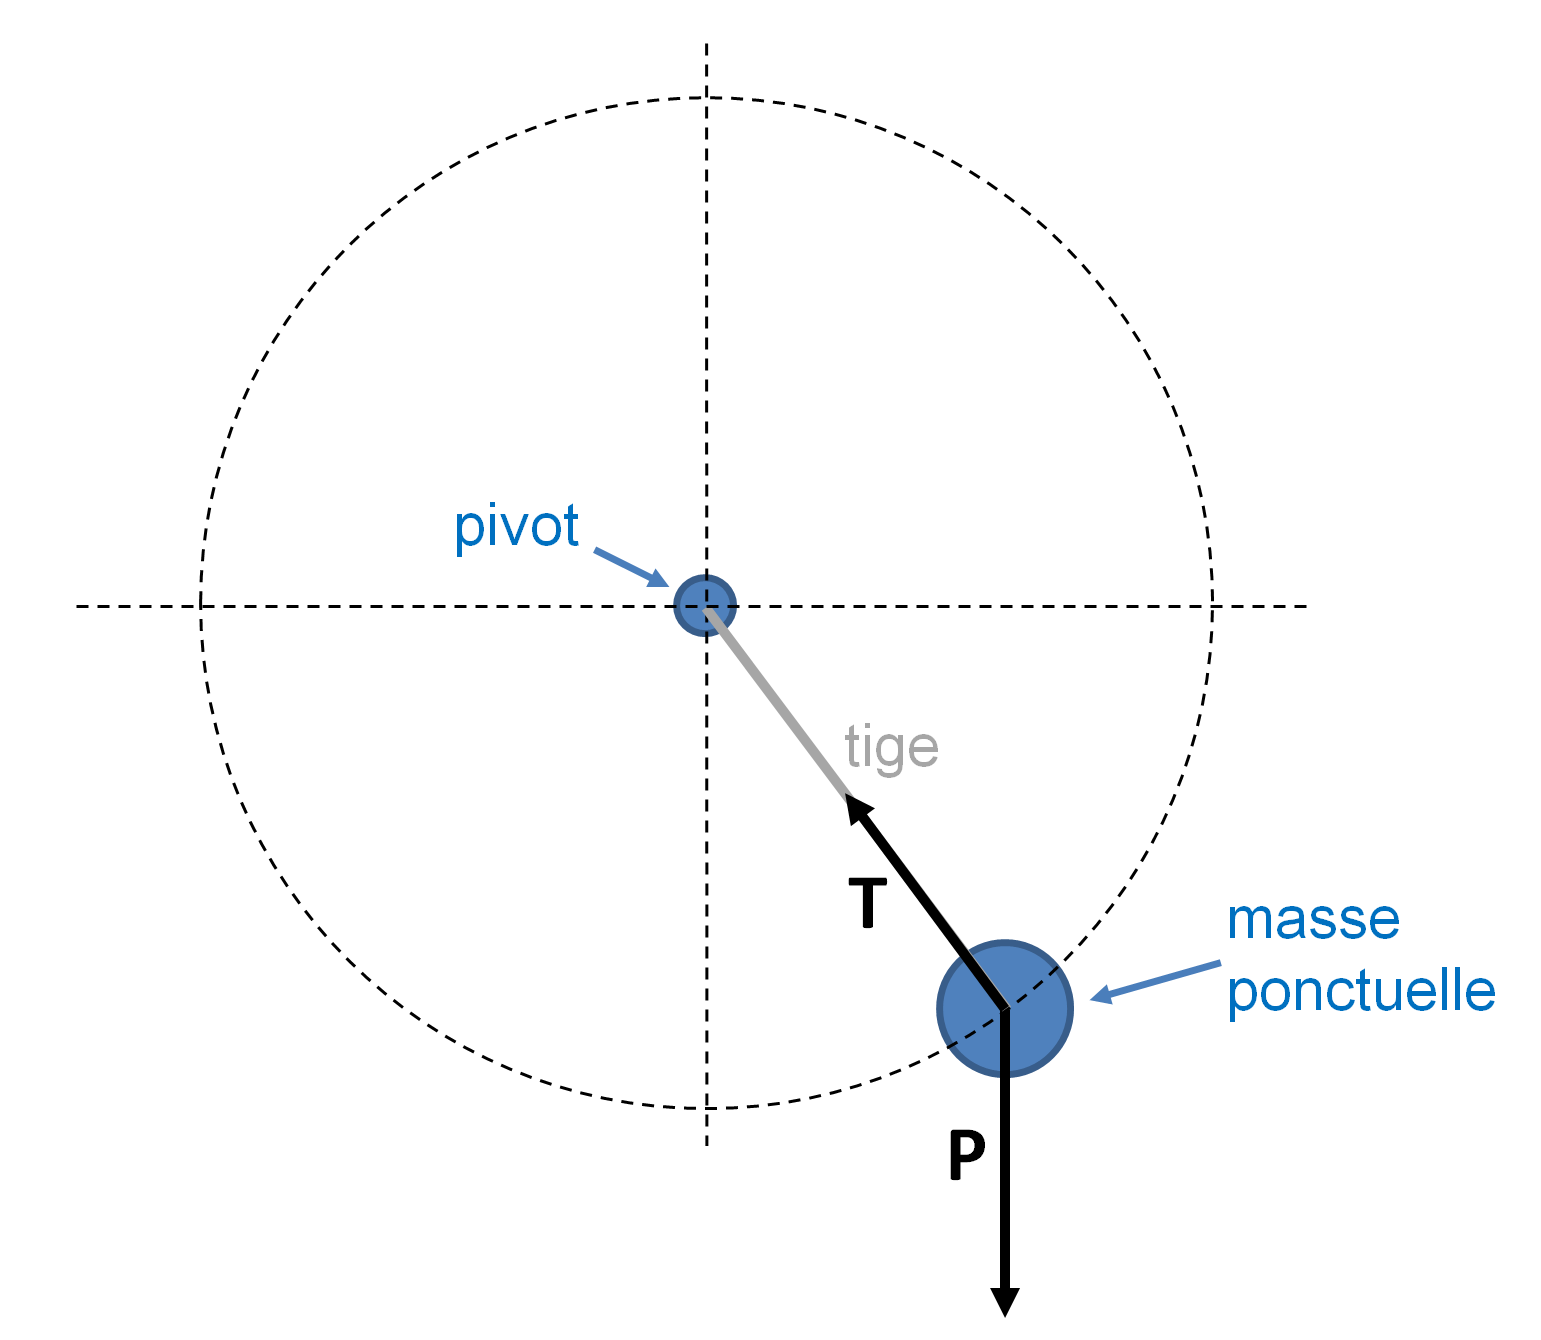
\includegraphics[width=0.80000\textwidth]{img/pendulum_sketch.png}
\caption{Bilan des forces dans un pendule
simple.\label{fig:pendulum_sketch}}
\end{figure}

La figure \ref{fig:pendulum_sketch2} montre un schéma des différentes
grandeurs caractérisant le pendule. La coordonnée naturelle pour définir
la position du pendule est l'angle \(\theta\). Nous verrons plus tard
comment convertir cet angle en coordonnées cartésiennes pour l'affichage
dans un \emph{canvas tkinter}. Nous choisissons de fixer \(\theta = 0\)
lorsque le pendule est à sa position d'équilibre. Il s'agit de la
position où la boule est au plus bas. C'est une position à laquelle le
pendule ne bougera pas s'il n'a pas une vitesse préexistante. Nous
choisissons par ailleurs de considérer \(\theta\) positif lorsque le
pendule se balance à droite, et négatif de l'autre côté. \textbf{g}
décrit l'accélération due à la gravité, avec
\(\boldsymbol{\mathbf P} = m \boldsymbol{\mathbf g}\), ou si on raisonne
en scalaire \(P = mg\). Les deux vecteurs représentant les composantes
tangentielle et orthogonale au mouvement du pendule de \textbf{P} sont
représentées sur le schéma (les annotations indiquent leur norme).

\begin{figure}[htbp]
\centering
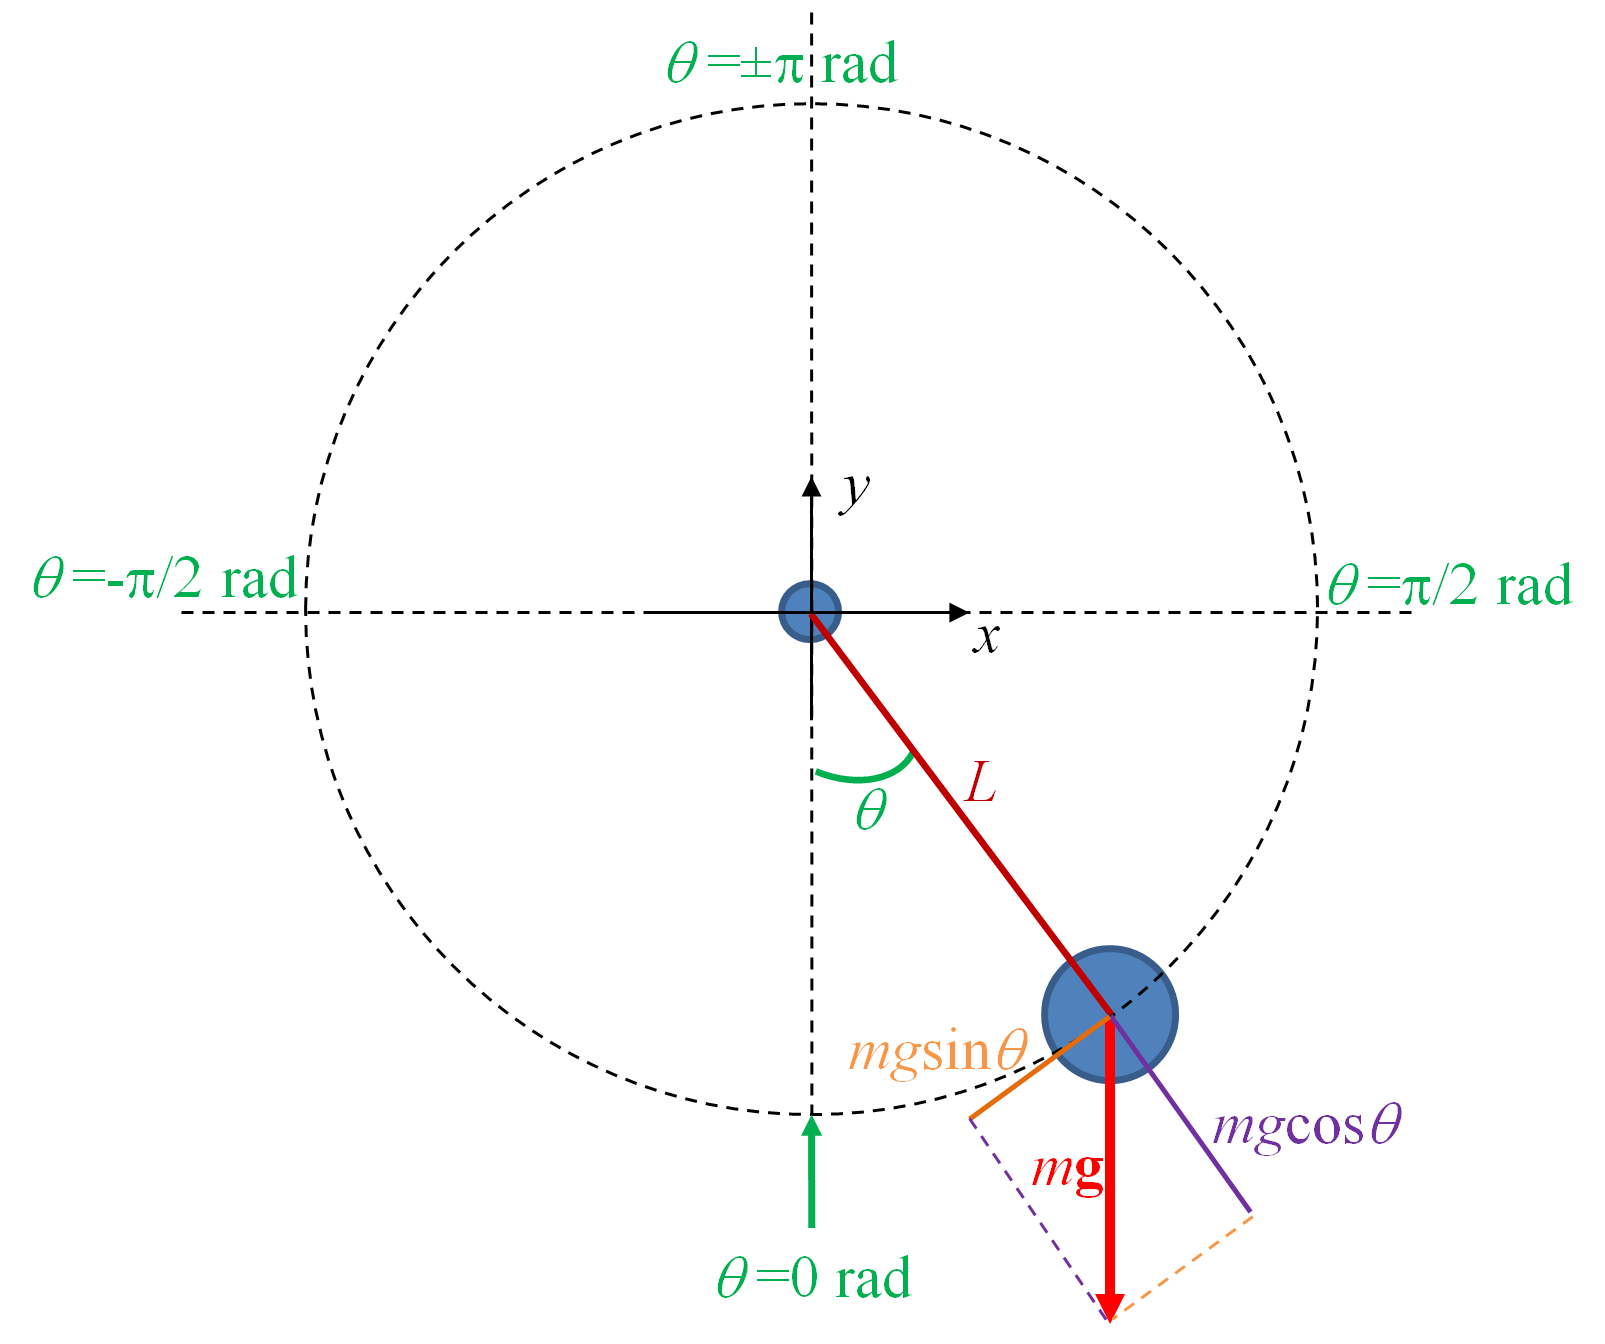
\includegraphics[width=0.80000\textwidth]{img/pendulum_sketch2.png}
\caption{Caractérisation géométrique d'un pendule
simple.\label{fig:pendulum_sketch2}}
\end{figure}

Si on déplace le pendule de sa position d'équilibre, il sera mû par la
force \textbf{F} résultant de la tension \textbf{T} et de son poids
\textbf{P} (cf.~plus bas). Comme le système est considéré comme parfait
(pas de frottement, gravité uniforme, etc.), le pendule ne s'arrêtera
jamais. Si on le monte à \(\theta = +20\) deg et qu'on le lâche, le
pendule redescendra en passant par \(\theta = 0\) deg, remontera de
l'autre côté à \(\theta = -20\) deg, puis continuera de la sorte
indéfiniment, grâce à la conservation de l'énergie dans un système fermé
(c'est-à-dire sans « fuite » d'énergie).

Ici, on va tenter de simuler ce mouvement en appliquant les
\href{https://fr.wikipedia.org/wiki/Lois_du_mouvement_de_Newton}{lois du
mouvement de Newton} et en résolvant les équations correspondantes
numériquement. D'après la seconde loi de Newton, la force (\textbf{F})
agissant sur la boule est égale à sa masse (\emph{m}) fois son
accélération (\textbf{a}) :

\[\boldsymbol{\mathbf F} = m \boldsymbol{\mathbf a}\]

Cette loi est exprimée ici dans le système de coordonnées cartésiennes
(le plan à 2 dimensions). La force \textbf{F} et l'accélération
\textbf{a} sont des vecteurs dont les composantes sont respectivement
\((F_{x}, F_{y})\) et \((a_{x}, a_{y})\). La force \textbf{F} correspond
à la somme vectorielle de \textbf{T} et \textbf{P}. La tige du pendule
étant rigide, le mouvement de la boule est restreint sur le cercle de
rayon égal à la longueur \emph{L} de la tige (dessiné en pointillé).
Ainsi, seule la composante tangentielle de l'accélération \textbf{a}
sera prise en compte dans ce mouvement. Comment la calculer ? La force
de tension \textbf{T} étant orthogonale au mouvement du pendule,
celle-ci n'aura pas d'effet. De même, la composante orthogonale
\(mgcos \theta\) due au poids \textbf{P} n'aura pas d'effet non plus. Au
final, on ne prendra en compte que la composante tangentielle due au
poids, c'est-à-dire \(mg sin \theta\) (cf.~figure
\ref{fig:pendulum_sketch2}). Au final, on peut écrire l'expression
suivante en raisonnant sur les valeurs scalaires :

\[F = ma = -mg sin \theta\]

Le signe \(-\) dans cette formule est très important. Il indique que
l'accélération s'oppose systématiquement à \(\theta\). Si le pendule se
balance vers la droite et que \(\theta\) devient plus positif,
l'accélération tendra toujours à faire revenir la boule dans l'autre
sens vers sa position d'équilibre à \(\theta = 0\). On peut faire un
raisonnement équivalent lorsque le pendule se balance vers la gauche et
que \(\theta\) devient plus négatif.

Si on exprime l'accélération en fonction de \(\theta\), on trouve ce
résultat qui peut sembler peu intuitif au premier abord :

\[a = -g sin \theta\]

Le mouvement du pendule ne dépend pas de sa masse !

Idéalement, nous souhaiterions résoudre cette équation en l'exprimant en
fonction de \(\theta\) seulement. Cela est possible en reliant
\(\theta\) à la longueur effective de l'arc \(s\) parcourue par le
pendule :

\[s = \theta L\]

Pour bien comprendre cette formule, souvenez-vous de la formule bien
connue du cercle \(l = 2 \pi r\) (où \emph{l} est la circonférence, et
\emph{r} le rayon) ! Elle relie la valeur de \(\theta\) à la distance de
l'arc entre la position actuelle de la boule et l'origine (à
\(\theta = 0\)). On peut donc exprimer la vitesse du pendule en dérivant
\(s\) par rapport au temps \(t\) :

\[v = \frac{ds}{dt} = L\frac{d \theta}{dt}\]

On peut aussi exprimer l'accélération \emph{a} en dérivant l'arc
\emph{s} deux fois par rapport à \emph{t} :

\[a = \frac{d^2s}{dt^2} = L\frac{d^2 \theta}{dt^2}\]

A nouveau, cette dernière formule exprime l'accélération de la boule
lorsque le mouvement de celle-ci est restreint sur le cercle pointillé.
Si la tige n'était pas rigide, l'expression serait différente.

Si on remplace \emph{a} dans la formule ci-dessus, on trouve :

\[L \frac{d^2 \theta}{dt^2} = -g sin \theta\]

Soit en remaniant, on trouve l'équation différentielle en \(\theta\)
décrivant le mouvement du pendule :

\[\frac{d^2 \theta}{dt^2} + \frac{g}{L} sin \theta = 0\]

Dans la section suivante, nous allons voir comment résoudre
numériquement cette équation différentielle.

\subsubsection{Résolution de l'équation différentielle du
pendule}\label{ruxe9solution-de-luxe9quation-diffuxe9rentielle-du-pendule}

Il existe de nombreuses
\href{https://en.wikipedia.org/wiki/Numerical_methods_for_ordinary_differential_equations}{méthodes
numériques de résolution d'équations différentielles}. L'objet ici n'est
pas de faire un rappel sur toutes ces méthodes ni de les comparer, mais
juste d'expliquer une de ces méthodes fonctionnant efficacement pour
simuler notre pendule.

Nous allons utiliser la
\href{https://en.wikipedia.org/wiki/Semi-implicit_Euler_method}{méthode
semi-implicite d'Euler}. Celle-ci est relativement intuitive à
comprendre.

Commençons d'abord par calculer l'accélération angulaire \(a_{\theta}\)
au temps \emph{t} en utilisant l'équation différentielle précédemment
établie :

\[a_{\theta}(t) = \frac{d^2 \theta}{dt^2}(t) = - \frac{g}{L} sin \theta(t)\]

L'astuce sera de calculer ensuite la vitesse angulaire au pas suivant
\(t + \delta t\) grâce à la relation :

\[v_{\theta}(t+\delta t) = \frac{d\theta}{dt}(t+\delta t) \approx v_{\theta}(t) + a_{\theta}(t) \times \delta t\]

Cette équation est ni plus ni moins qu'un remaniement de la définition
de l'accélération, à savoir, la variation de vitesse par rapport à un
temps. Cette vitesse \(v_{\theta}(t+\delta t)\) permettra au final de
calculer \(\theta\) au temps \(t + \delta t\) (c'est-à-dire ce que l'on
cherche !) :

\[\theta (t + \delta t) \approx \theta (t) + v_{\theta}(t+\delta t) \times \delta t\]

Dans une réalisation algorithmique, il suffira d'initialiser les
variables de notre système puis de faire une boucle sur un nombre de pas
de simulation. A chaque pas, on calculera \(a_{\theta}(t)\), puis
\(v_{\theta}(t+\delta t)\) et enfin \(\theta (t + \delta t)\) à l'aide
des formules ci-dessus.

L'initialisation des variables pourra ressembler à cela :

\begin{verbatim}
L <- 1          # longueur tige en m
g <- 9.8        # accélération gravitationnelle en m/s^2
t <- 0          # temps initial en s
dt <- 0.05      # pas de temps en s
# conditions initiales
theta <- pi / 4 # angle initial en rad
dtheta <- 0     # vitesse angulaire initiale en rad/s

afficher_position_pendule(t, theta) # afficher position de départ
\end{verbatim}

L'initialisation des valeurs de \texttt{theta} et \texttt{dtheta} est
très importante car elle détermine le comportement du pendule. Nous
avons choisi ici d'avoir une vitesse angulaire nulle et un angle de
départ du pendule \(\theta = \pi / 4\) rad \(= 45\) deg. Le pas
\texttt{dt} est également très important, c'est lui qui déterminera
l'erreur faite sur l'intégration de l'équation différentielle. Plus ce
pas est petit, plus on est précis, mais plus le calcul sera long. Ici,
on choisit un pas \texttt{dt} de 0.05 s qui constitue un bon compromis.

A ce stade, vous avez tous les éléments pour tester votre pendule.
Essayez de réaliser un petit programme python \texttt{pendule\_basic.py}
qui utilise les conditions initiales ci-dessus et simule le mouvement du
pendule. A la fin de cette rubrique, nous proposons une solution en
langage algorithmique. Essayez dans un premier temps de le faire
vous-même. A chaque pas, le programme écrira le temps \(t\) et l'angle
\(\theta\) dans un fichier \texttt{pendule\_basic.dat}. Dans les
équations, \(\theta\) doit être exprimé en radian, mais nous vous
conseillons de convertir cet angle en degré dans le fichier (plus facile
à comprendre pour un humain !). Une fois ce fichier généré, vous pourrez
observer le graphe correspondant avec \emph{matplotlib} en utilisant le
code suivant :

\begin{verbatim}
import matplotlib.pyplot as plt
import numpy as np

# la fonction np.genfromtxt() renvoie un array à 2 dim
array_data = np.genfromtxt("pendule_basic.dat")
# col 0: t, col 1: theta
t = array_data[:,0]
theta = array_data[:,1]

# plot
plt.figure(figsize=(8,8))
mini = min(theta) * 1.2
maxi = max(theta) * 1.2
plt.xlim(0, max(t))
plt.ylim(mini, maxi)
plt.xlabel('t (s)')
plt.ylabel('theta (deg)')
plt.plot(t, theta)
plt.savefig("pendule_basic.png")
\end{verbatim}

Si vous observez une sinusoïde, bravo, vous venez de réaliser votre
première simulation de pendule ! Vous avez maintenant le « squelette »
de votre « moteur » de simulation. N'hésitez pas à vous amuser avec
d'autres conditions initiales. Ensuite vous pourrez passer à la rubrique
suivante.

Si vous avez bloqué dans l'écriture de la boucle, voici à quoi elle
pourrait ressembler en langage algorithmique :

\begin{verbatim}
tant qu'on n'arrête pas le pendule:
    # acc angulaire au tps t (en rad/s^2)
    d2theta <- -(g/L) * sin(theta)
    # v angulaire mise à jour de t -> t + dt
    dtheta <- dtheta + d2theta * dt
    # theta mis à jour de t -> t + dt
    theta <- theta + dtheta * dt
    # t mis à jour
    t <- t + dt
    # mettre à jour l'affichage
    afficher_position_pendule(t, theta)
\end{verbatim}

\subsubsection{\texorpdfstring{Constructeur de l'application en
\emph{tkinter}}{Constructeur de l'application en tkinter}}\label{constructeur-de-lapplication-en-tkinter}

Nous allons maintenant construire l'application \emph{tkinter} en vous
guidant pas à pas. Il est bien sûr conseillé de relire le chapitre 20
sur \emph{tkinter} avant de vous lancer dans cette partie.

Comme expliqué largement dans le chapitre 20, nous allons construire
l'application avec une classe. Le programme principal sera donc très
allégé et se contentera d'instancier l'application, puis de lancer le
gestionnaire d'événements :

\begin{verbatim}
if __name__ == "__main__":
    """Programme principal (instancie la classe principale, donne un
    titre et lance le gestionnaire d'événements)
    """
    app_pendule = AppliPendule()
    app_pendule.title("Pendule")
    app_pendule.mainloop()
\end{verbatim}

Ensuite, nous commençons par écrire le constructeur de la classe. Dans
ce constructeur, nous aurons une section initialisant toutes les
variables utilisées pour simuler le pendule (cf.~rubrique précédente),
puis, une autre partie générant les \emph{widgets} et tous les éléments
graphiques. Nous vous conseillons vivement de bien les séparer, et
surtout de \textbf{mettre des commentaires} pour pouvoir s'y retrouver.
Voici un « squelette » pour vous aider :

\begin{verbatim}
class AppliPendule(tk.Tk):
    def __init__(self):
        # instanciation de la classe Tk
        tk.Tk.__init__(self)
        # ici vous pouvez définir toutes les variables
        # concernant la physique du pendule
        self.theta = np.pi / 4 # valeur intiale theta
        self.dtheta = 0 # vitesse angulaire initiale
        [...]
        self.g = 9.8 # cst gravitationnelle en m/s^2
        [...]
        # ici vous pouvez construire l'application graphique
        self.canv = tk.Canvas(self, bg='gray', height=400, width=400)
        # création d'un boutton demarrer, arreter, quitter
        # penser à placer les widgets avec .pack()
        [...]
\end{verbatim}

La figure \ref{fig:pendule} vous montre un aperçu de ce que l'on
voudrait obtenir.

\begin{figure}[htbp]
\centering
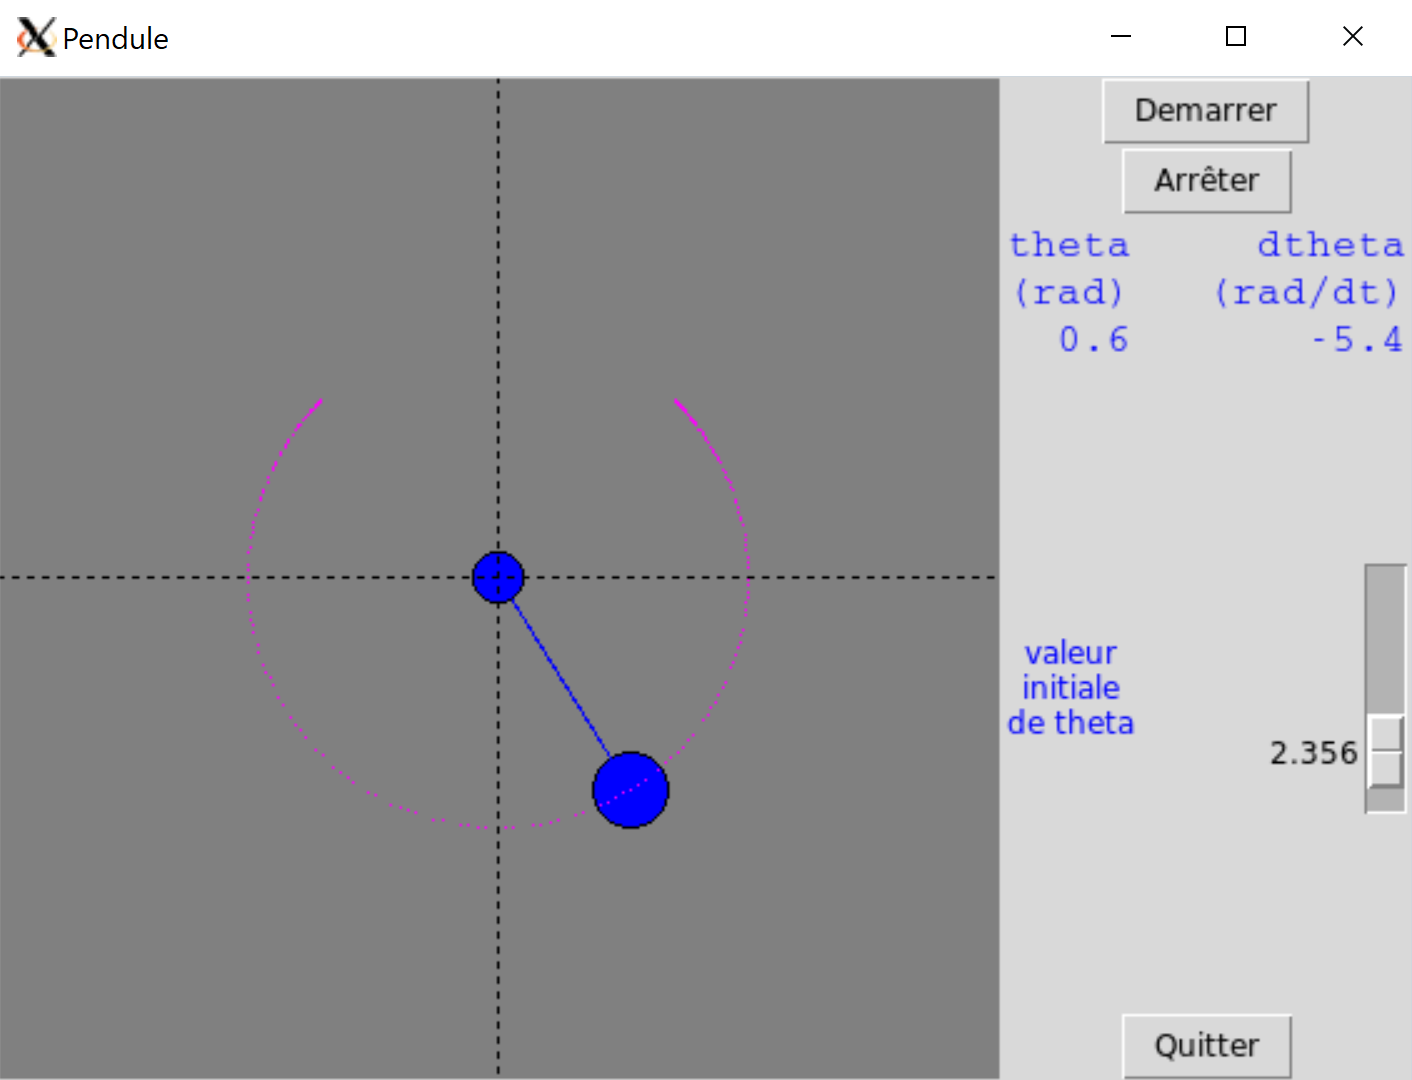
\includegraphics[width=0.60000\textwidth]{img/pendule.png}
\caption{Application pendule.\label{fig:pendule}}
\end{figure}

Pour le moment, vous pouvez oublier la réglette fixant la valeur
initiale de \(\theta\), les \emph{labels} affichant la valeur de
\(\theta\) et \(v_{\theta}\) ainsi que les points violets « laissés en
route » par le pendule. De même, nous dessinerons le pivot, la boule et
la tige plus tard. A ce stade, il est fondamental de tout de suite
lancer votre application pour vérifier que les \emph{widgets} sont bien
placés. N'oubliez pas, un code complexe se teste \textbf{au fur et à
mesure} lors de son développement.

\emph{Conseil} : pour éviter un message d'erreur si toutes les méthodes
n'existe pas encore, vous pouvez indiquer \texttt{command=self.quit}
pour chaque bouton (vous le changerez après).

\subsubsection{Créations des dessins dans le
canvas}\label{cruxe9ations-des-dessins-dans-le-canvas}

Le pivot et la boule pourront être créés avec la méthode
\texttt{.create\_oval()}, la tige le sera avec la méthode
\texttt{.create\_line()}. Pensez à créer des variables pour la tige et
la boule lors de l'instanciation car celles-ci bougeront par la suite.

Comment placer ces éléments dans le \emph{canvas} ? Vous avez remarqué
que lors de la création de ce dernier, nous avons fixé une dimension de
400 \(\times\) 400 pixels. Le pivot se trouve au centre, c'est-à-dire au
point \((200, 200)\) . Pour la tige et la boule il sera nécessaire de
connaître la position de la boule cette dernière \textbf{dans le repère
du canvas}. Or, pour l'instant, nous définissons la position de la boule
avec l'angle \(\theta\). Il va donc nous falloir convertir \(\theta\) en
coordonnées cartésiennes \((x, y)\) dans le repère mathématique défini
dans la figure \ref{fig:pendulum_sketch2}, puis dans le repère du
\emph{canvas} \((x_{c}, y_{c})\) (cf.~rubrique suivante).

\paragraph{\texorpdfstring{Conversion de \(\theta\) en coordonnées
\((x, y)\)}{Conversion de \textbackslash{}theta en coordonnées (x, y)}}\label{conversion-de-theta-en-coordonnuxe9es-x-y}

Cette étape est relativement simple si on considère le pivot comme le
centre du repère. Avec les fonctions trigonométriques \texttt{sin()} et
\texttt{cos()}, vous pourrez calculer la position de la boule
(cf.~exercice sur la spirale dans le chapitre 7). Faites attention
toutefois aux deux aspects suivants :

\begin{itemize}
\tightlist
\item
  la trajectoire de la boule suit les coordonnées d'un cercle de rayon
  \emph{L} (si on choisit \emph{L} = 1 m, ce sera plus simple) ;
\item
  nous sommes décalés par rapport au cercle trigonométrique classique ;
  si on considère \emph{L} = 1 m :

  \begin{itemize}
  \tightlist
  \item
    quand \(\theta = 0\), on a le point \((0, -1)\) ;
  \item
    quand \(\theta = + \pi / 2 = 90\) deg, on a \((1, 0)\) ;
  \item
    quand \(\theta = - \pi / 2 = -90\) deg, on a \((-1, 0)\) ;
  \item
    quand \(\theta = \pm \pi = \pm 180\) deg, on a \((0, 1)\).
  \end{itemize}
\end{itemize}

Si vous n'avez pas trouvé, voici la solution :

\begin{verbatim}
self.x = np.sin(self.theta) * self.L
self.y = -np.cos(self.theta) * self.L
\end{verbatim}

\paragraph{\texorpdfstring{Méthode convertissant \(\theta\) en
coordonnées
\((x, y)\)}{Méthode convertissant \textbackslash{}theta en coordonnées (x, y)}}\label{muxe9thode-convertissant-theta-en-coordonnuxe9es-x-y}

Il nous faut maintenant convertir \((x, y)\) en coordonnées
\((x_{c}, y_{c})\) dans le \emph{canvas}. Plusieurs choses sont
importantes pour cela :

\begin{itemize}
\tightlist
\item
  le centre du repère mathématique \((0, 0)\) a la coordonnée
  \((200, 200)\) dans le \emph{canvas} ;
\item
  il faut choisir un facteur de conversion : par exemple, si on choisit
  \emph{L} = 1 m, on peut proposer le facteur 1 m \(\rightarrow\) 100
  pixels ;
\item
  l'axe des ordonnées dans le \emph{canvas} est \textbf{inversé} par
  rapport au repère mathématique.
\end{itemize}

open-box-adv

Il est essentiel d'écrire une méthode qui convertira \(\theta\) en
\((x, y)\) puis \((x_{c}, y_{c})\) dans votre classe. Vous pouvez
l'appeler par exemple \texttt{.theta2xc\_yc()}.

close-box-adv

Si vous n'avez pas trouvé, voici la solution :

\begin{verbatim}
self.conv_factor = 100
self.x_c = self.x*self.conv_factor + 200
self.y_c = -self.y*self.conv_factor + 200
\end{verbatim}

TODO:

\begin{itemize}
\tightlist
\item
  mouvement du pendule: mth .start(), .stop(), .move() (se référer à la
  baballe)
\end{itemize}

\subsubsection{Ressource
complémentaire}\label{ressource-compluxe9mentaire}

Si vous souhaitez aller plus loin sur les différentes méthodes
numériques de résolution d'équation différentielle associées au pendule,
nous vous conseillons le site de
\href{http://pages.physics.cornell.edu/~sethna/StatMech/ComputerExercises/Pendulum/Pendulum.html}{James
Sethna} de l'université de Cornell.

\end{document}
